\begin{figure*}[t]
\vskip 0.2in
\begin{center}
\centerline{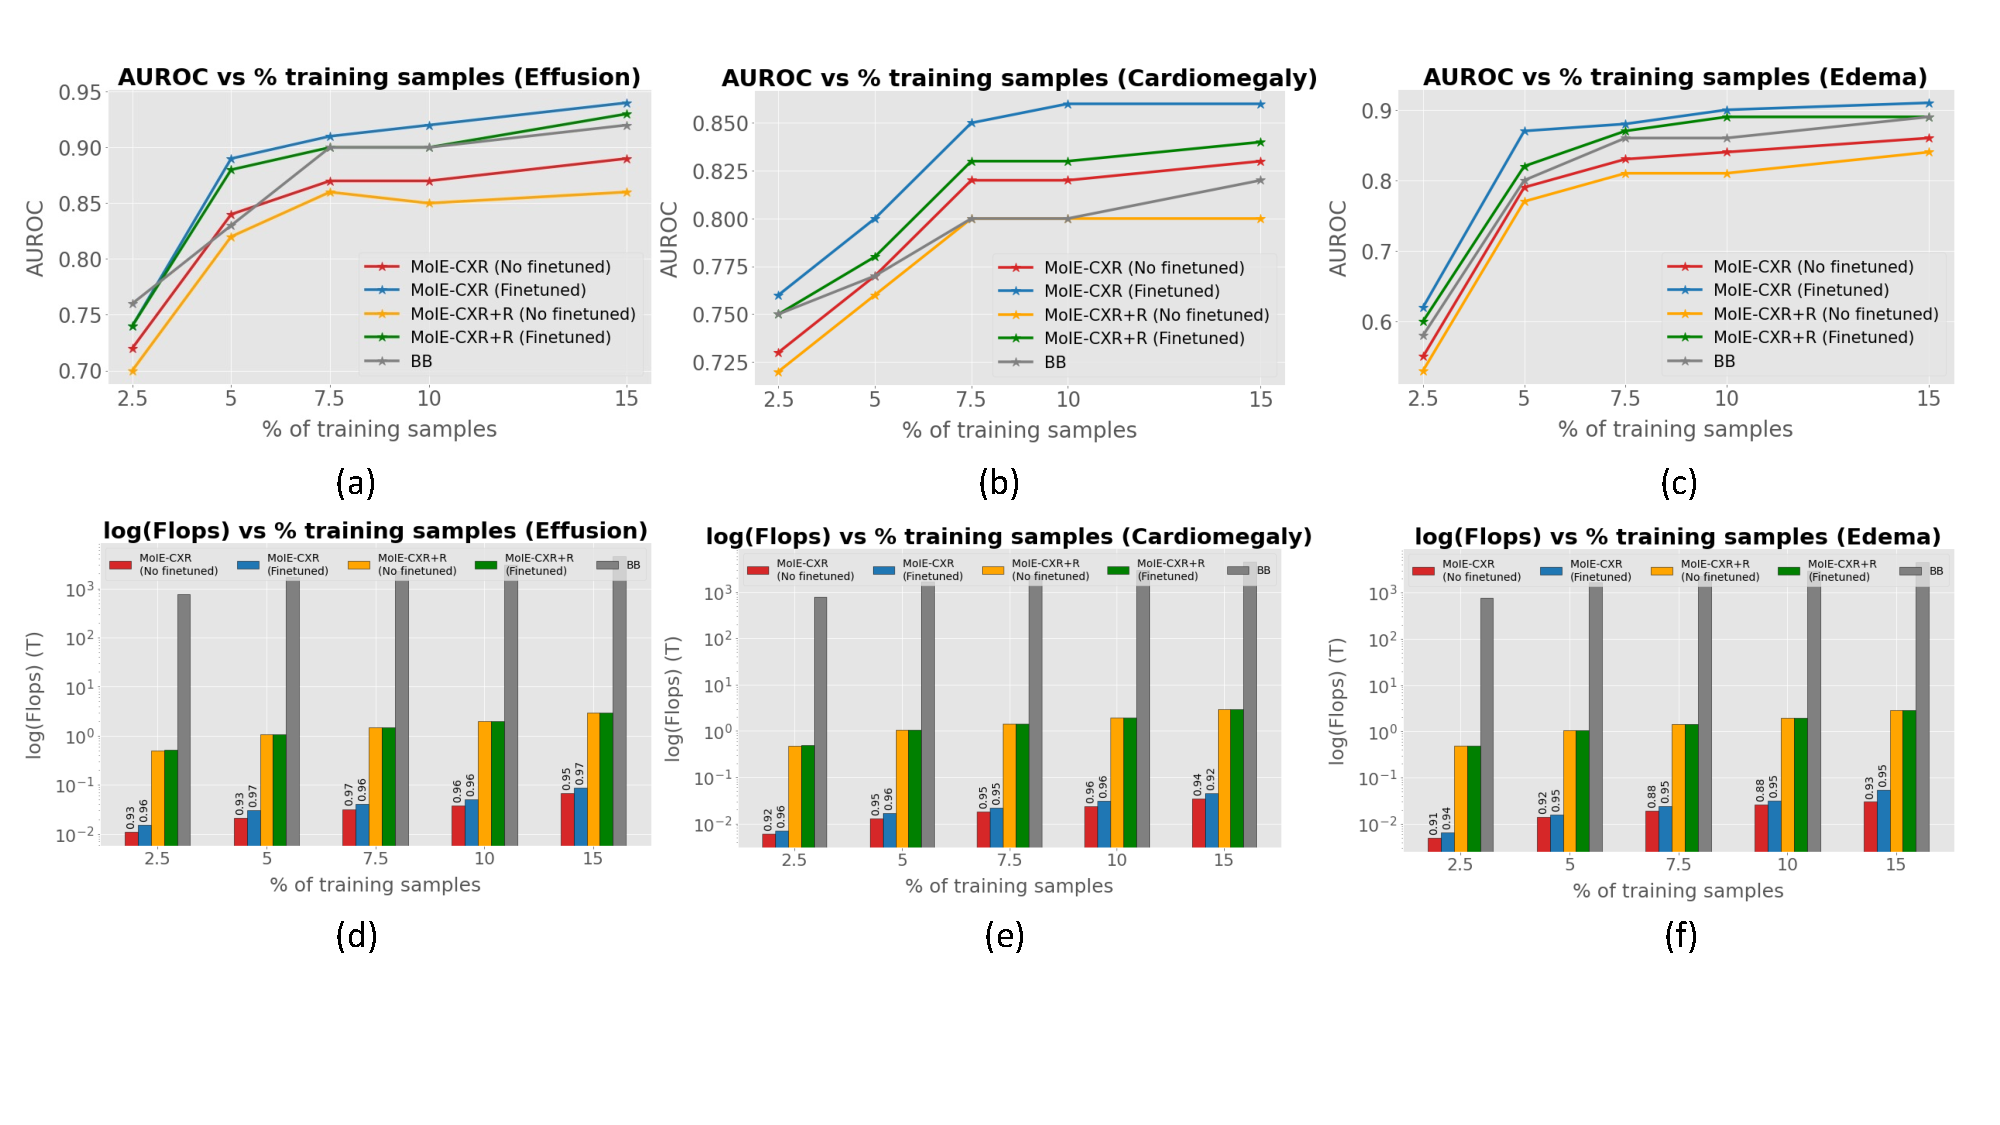
\includegraphics[width=\linewidth]{plots/main/Domain_genelization.pdf}}
\caption{Transfering the first 3 experts of MoIE-CXR trained on MIMIC-CXR to Stanford-CXR. With varying \% of training samples of Stanford CXR, \textbf{(a-c):}  reports AUROC of the test sets, \textbf{(d-g)} reports computation costs in terms of $\log\text{(Flops) (T)}$.
We report the coverages in Stanford-CXR on top of the ``finetuned'' and ``No finetuned'' variants of MoIE-CXR (red and blue bars) in \textbf{(d-g)}.
% The ``No finetuned'' variant of MoIE-CXR represents the model obtained only by finetuning selectors ($\pi$), not the experts ($g$). Similarly, the ``Finetuned'' MoIE-CXR represents the model obtained by jointly finetuning $\pi$ and $g$ for 5 epochs.
}
\label{fig:domain_generelization}
\end{center}
\end{figure*}

\noindent \textbf{Applying MoIE-CXR to the unseen domain.} In this experiment, we utilize Algo.~\ref{algo: domain_transfer} to transfer MoIE-CXR trained on MIMIC-CXR dataset to Stanford Chexpert~\cite{irvin2019chexpert} dataset for the diseases -- effusion, cardiomegaly and edema. Using 2.5\%, 5\%, 7.5\%, 10\%, and 15 \% of training data from the Stanford Chexpert dataset, we employ two variants of MoIE-CXR where we (1) train only the selectors ($\pi$) without finetuning the experts ($g$) (``No finetuned'' variant of MoIE-CXR in Fig.~\ref{fig:domain_generelization}), and (2) finetune $\pi$ and $g$ jointly for only 5 epochs (``Finetuned'' variant of MoIE-CXR and MoIE-CXR + R in Fig.~\ref{fig:domain_generelization}). Finetuning $\pi$ is essential to route the samples of the target domain to the appropriate expert. As later experts cover the ``harder'' samples of MIMIC-CXR, we only transfer the experts of the first three iterations (refer to Fig.~\ref{fig:expert_performance_cv_vit}). To ensure a fair comparison, we finetune (both the feature extractor $\Phi$ and classifier $h^0$) BB: $f^0 = h^0 \circ \Phi$ of MIMIC-CXR with the same training data of Stanford Chexpert for 5 epochs. Throughout this experiment, we fix $\Phi$ while finetuning the final residual in MoIE+R as stated in Eq.~\ref{equ: residual}. Fig.~\ref{fig:domain_generelization} displays the performances of different models and the computation costs in terms of Flops. The Flops are calculated as, Flop of (forward propagation + backward propagation) $\times$ (total no. of batches) $\times$ (no of training epochs). The finetuned MoIE-CXR outperforms the finetuned BB (on average $\sim 5\% \uparrow$ for effusion and cardiomegaly).
As experts are simple models~\cite{barbiero2022entropy} and accept only low dimensional concept vectors compared to BB, the computational cost to train MoIE-CXR is significantly lower than that of BB (Fig.~\ref{fig:domain_generelization} (d-f)). Specifically, BB requires $\sim$ 776T flops to be finetuned on 2.5\% of the training data of Stanford CheXpert, whereas MoIE-CXR requires $\sim$ 0.0065T flops. As MoIE-CXR discovers the sample-specific domain-invariant concepts, it achieves such high performance with low computational cost than BB. 
